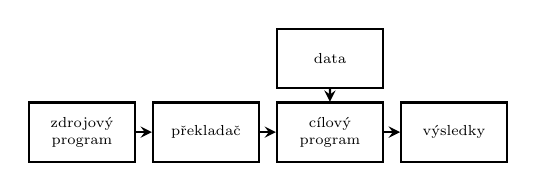
\begin{tikzpicture}[
    scale=0.75,
    transform shape,
    box/.style={
        draw,
        thick,
        minimum width=18mm,
        minimum height=10mm,
        align=center,
        font=\scriptsize
    },
    arrow/.style={->, thick, >=stealth}
]
    \node[box] (src) at (0,0) {zdrojový\\program};
    \node[box] (comp) at (2.1,0) {překladač};
    \node[box] (target) at (4.2,0) {cílový\\program};
    \node[box] (data) at (4.2,1.25) {data};
    \node[box] (out) at (6.3,0) {výsledky};

    \draw[arrow] (src) -- (comp);
    \draw[arrow] (comp) -- (target);
    \draw[arrow] (target) -- (out);
    \draw[arrow] (data) -- (target);
\end{tikzpicture}
